\section{Milestone I}\label{sec:milestone_1}
Some introduction about what it is all about.

Cite: \citet{baumannLectureNotesCosmology2017} or \citet{dodelsonModernCosmology2021} \citep{callinHowCalculateCMB2006, wintherCosmologyIILecture2024, huCompleteTreatmentCMB1998}

\subsection{Theory}
The theory behind this milestone. See Friedmann equation \ref{eq:Friedmann}

Fiducial cosmology and initial parameter values taken from Planck 2018 results \citep{collaborationPlanck2018Results2020}.

\begin{equation}\label{eq:Friedmann}
    \boxed{H = H_0 \sqrt{ \Omega_{M 0} a^{-3} + \Omega_{R 0} a^{-4} + \Omega_{k 0} a^{-2} + \Omega_{\Lambda 0}}},
\end{equation}

where the $\Omega_{X}$ are density parameters describing relative density of their respective form of energy contributing to the expansion of the universe. Subscript $_0$ indicates a value for the universe of today, since we as observers are by definition at $x=a=z=0$.

$\Omega_{M 0} = (\Omega_{b0}+\Omega_{\rm CDM 0})$ is a composite density parameter describing non-relativistic matter, and $\Omega_{R 0} = (\Omega_{\gamma 0} + \Omega_{\nu 0})$ is a composite density term for radiation.

Paper with supernova fitting data \citet{betouleImprovedCosmologicalConstraints2014}

Equation for critical density of the universe today \ref{eq:critical_density}

\begin{equation}\label{eq:critical_density}
\rho_{c0} \equiv \frac{3H_0^2}{8\pi G}
\end{equation}

\subsection{Implementation details}
Something about the numerical work.

\subsection{Results}
Show and discuss the results.

See figs. \ref{fig:milestone_1_cosmic_vs_conformal_time}, \ref{fig:milestone_1_luminosity_distance}, \ref{fig:milestone_1_etaHp_over_c_of_x}, \ref{fig:milestone_1_Omega_i_of_x}, \ref{fig:milestone_1_supernovafitting_confidence_regions}.

\begin{figure}
\centering
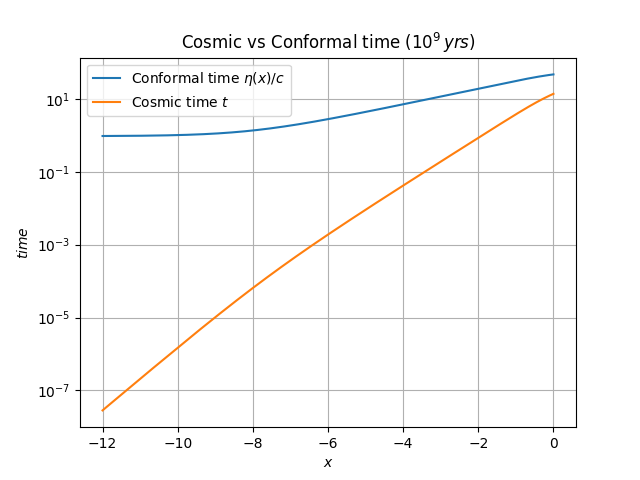
\includegraphics[width=0.4\textwidth]{../Milestone 1/Plots/cosmic_vs_conformal_time.png}
\caption{Caption}
\label{fig:milestone_1_cosmic_vs_conformal_time}
\end{figure}

\begin{figure}
\centering
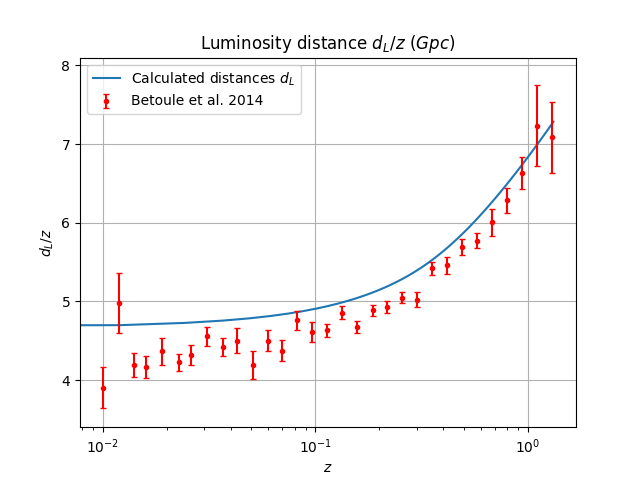
\includegraphics[width=0.4\textwidth]{../Milestone 1/Plots/luminosity_distance.png}
\caption{Caption}
\label{fig:milestone_1_luminosity_distance}
\end{figure}

\begin{figure}
\centering
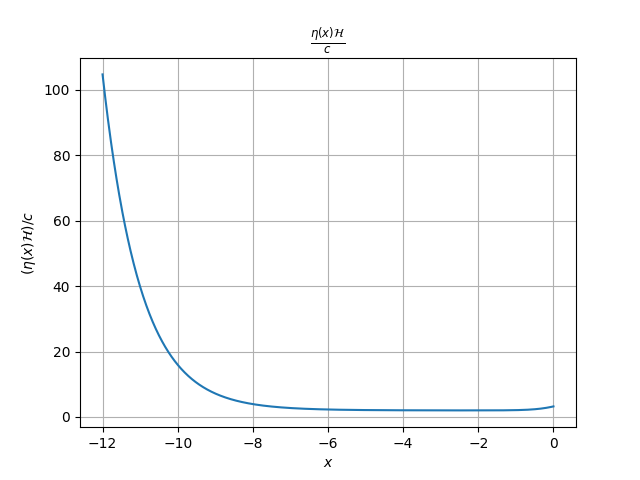
\includegraphics[width=0.4\textwidth]{../Milestone 1/Plots/etaHp_over_c_of_x.png}
\caption{Caption}
\label{fig:milestone_1_etaHp_over_c_of_x}
\end{figure}

\begin{figure}
\centering
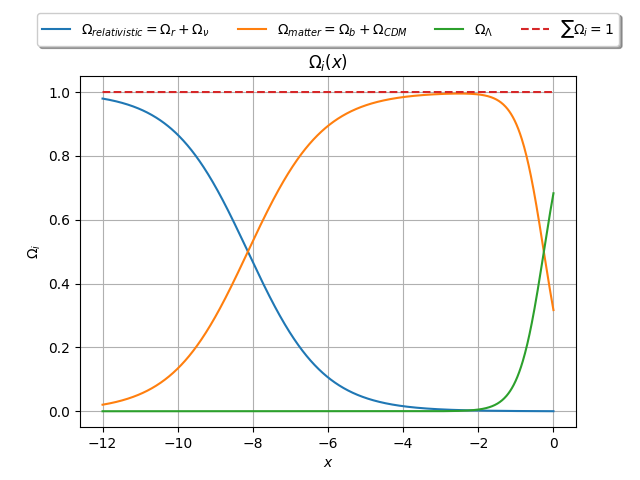
\includegraphics[width=0.4\textwidth]{../Milestone 1/Plots/Omega_i_of_x.png}
\caption{Caption}
\label{fig:milestone_1_Omega_i_of_x}
\end{figure}

\begin{figure}
\centering
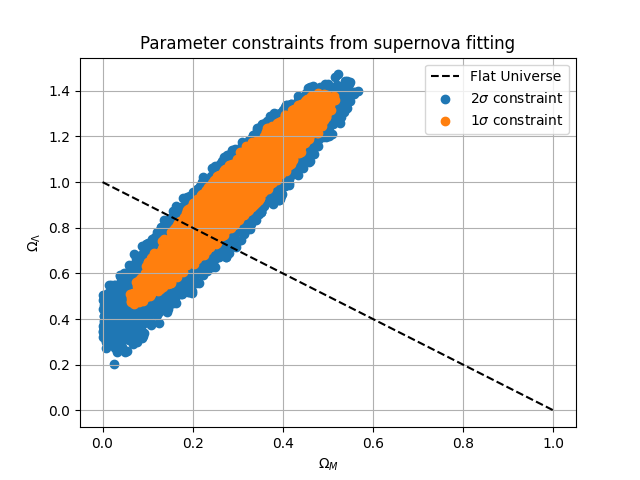
\includegraphics[width=0.4\textwidth]{../Milestone 1/Plots/supernovafitting_confidence_regions.png}
\caption{Caption}
\label{fig:milestone_1_supernovafitting_confidence_regions}
\end{figure}
